\documentclass[11pt]{article}

% ==== PACKAGES ==== %
% \usepackage{fullpage}
\usepackage{amsmath,amssymb,amsthm}
\usepackage{epic}
\usepackage{eepic}
\usepackage{hyperref}
\usepackage{listings}
\usepackage{float}
\usepackage{graphicx}
\usepackage{fancyhdr}
\usepackage{color}
\usepackage{bbm}
\usepackage[letterpaper, margin=1in]{geometry}

% ==== MARGINS ==== %
% \pagestyle{empty}
% \setlength{\oddsidemargin}{0in}
% \setlength{\textwidth}{6.8in}
% \setlength{\textheight}{9.5in}

\pagestyle{fancy}
\fancyhf{}
\rhead{ASEN 5044}
\lhead{Midterm 2}
\rfoot{Page \thepage}


\newtheorem*{solution*}{Solution}
\newtheorem{lemma}{Lemma}[section]
\newtheorem{theorem}[lemma]{Theorem}
\newtheorem{claim}[lemma]{Claim}
\newtheorem{definition}[lemma]{Definition}
\newtheorem{corollary}[lemma]{Corollary}
\lstset{moredelim=[is][\bfseries]{[*}{*]}}

% ==== DOCUMENT PROPER ==== %
\begin{document}

\thispagestyle{empty}

% --- Header Box --- %
\newlength{\boxlength}\setlength{\boxlength}{\textwidth}
\addtolength{\boxlength}{-4mm}

\begin{center}\framebox{\parbox{\boxlength}{\bf
      Statistical Estimation \hfill Midterm 2\\
      ASEN 5044 Fall 2018 \hfill Due Date: Nov 15, 2018\\
      Name: Andrew Kramer \hfill PhD Student
}}
\end{center}

\section*{Problem 1}
Suppose that a dynamic scalar system is given as $x_{k+1}=f_{x_k}+w_k$ where $w_k$ is zero-mean white noise with variance $q$. Show that if the variance of $x_k$ is $\sigma^2$ for all $k$, then it must be true that $f^2=(\sigma^2-q)/\sigma^2$. \textbf{Hint:} The problem says the variance of $x_k$ is $\sigma^2$ for all time steps $k$. It does \textit{not} say $x_k$ is zero mean for all $k$.

\subparagraph*{}
If we start with the assumption that $x_k\sim\mathcal{N}(\mu_k,\sigma^2)$ and $w_k\sim\mathcal{N}(0,q)$, then we can find the variance of $x_{k+1}$ as the variance of the linear combination $fx_k+w_k$:
\begin{equation*}
	\sigma_{x_{k+1}}^2 = f^2\sigma_{x_k}^2 + q
\end{equation*}
But since $x_k$ has the same variance at all timesteps $k$ the expression becomes $\sigma^2=f^2\sigma^2+q$. If we solve this equation for $f^2$ we get
\begin{equation*}
	f^2 = \frac{\sigma^2-q}{\sigma^2}
\end{equation*}

\section*{Problem 2}
Given the random vector $x\in\mathbb{R}^n$ (with some finite mean and covariance matrix) and the constant non-random matrix $A\in\mathbb{R}^{n\times n}$ where $A=A^T$, find $\mathbb{E}[x^TAx]$. Be sure to show and properly explain all steps used to get your result. \textbf{Hint:} Ref lecture 2, slide 2. Think about the size of the result of the quadratic form to see the relevant connection. To use this fact, you should first prove that, if $Z$ is a square matrix whose elements are random variables then $\mathbb{E}[\text{tr}(AZ)]=\text{tr}(A\mathbb{E}[Z])$.

\subparagraph*{}
$\mathbb{E}[x^TAx]$ can be broken down as follows:
\begin{align*}
	\mathbb{E}[x^TAx] &= \mathbb{E}\Bigg[\sum_{i=1}^n\sum_{j=1}^n a_{ij}x_ix_j\Bigg] \\
	&= \sum_{i=1}^n\sum_{j=1}^na_{ij}\mathbb{E}[x_ix_j]\\
	&= \sum_{i=1}^n\sum_{j=1}^na_{ij}\Bigg[\text{cov}(x_i,x_j)+\mathbb{E}[x_i]\mathbb{E}[x_j]\Bigg] \\
	&= \sum_{i=1}^n\sum_{j=1}^n a_{ij}(\sigma_{ji}+\mu_i\mu_j)\quad \text{noting: } \text{cov}(x_i,x_j)=\text{cov}(x_j,x_i)\\
	&= \sum_{i=1}^n\sum_{j=1}^n a_{ij}\sigma_{ji} + \sum_{i=1}^n\sum_{j=1}^n a_{ij}\mu_i\mu_j \\
	&= \text{tr}(AP) + \mu^TA\mu
\end{align*}
where $\sigma_{ij}$ is the covariance between $x_i$ and $x_j$, $P$ is the full covariance matrix of $x$, and $\mu$ is the expected value of $x$.

\section*{Problem 3}
Consider the coordinated turning aircraft problem from homework 7. Assume again the dynamics are free of process noise,
\begin{equation*}
	x(k+1)=Fx(k)
\end{equation*}
for the $F$ matrix and states as defined in homework 7 for some unknown turning rate $\Omega$ and discretization step $\Delta T$. Now add measurements of the form 
\begin{align*}
	y(k+1)&=Hx(k+1)+v(k+1) \\
	\mathbb{E}[v(k)] &= 0,\quad \mathbb{E}[v(k)v(j)^T] = \delta(k,j)R(k)
\end{align*}
with additive white noise $v(k)$ and non-stationary noise covariance $R(k)$. For each part of this problem, it is desired to estimate the initial state $x(0)\in\mathbb{R}^n$ of a dynamical system consisting of either one or two turning aircraft at time $k=0$ from noisy measurements $y(k)\in\mathbb{R}^p$ taken at time steps $k=1,2,\dots,T$.

\subsection*{part (a)}
Derive an analytical expression for the batch estimator $\hat{x}(0)$ which minimizes the cost function
\begin{equation*}
	J(T)=\sum_{k=1}^T(y_k-\hat{y}_k)^T[R(k)]^{-1}(y_k-\hat{y}_k)
\end{equation*}
where $\hat{y}_k$ is the time $k$ estimator-based predicted measurement (a function of $\hat{x}(0)$) and $y_k$ is the actual measurement at time $k$. Be sure to precisely and carefully define all matrices and vectors used by the estimator, for the case where $x_k$ and $y_k$ obey equations (1) and (2).

\subparagraph*{}
The cost function is
\begin{align*}
	J(T) &= \sum_{k=1}^T(y_k-\hat{y}_k)^T[R(k)]^{-1}(y_k-\hat{y}_k) \\
	&= \sum_{k=1}^T(y_k-Hx(k))^T[R(k)]^{-1}(y_k-Hx(k)) \\
	&= \sum_{k=1}^T(y_k-HF^kx(0))^T[R(k)]^{-1}(y_k-HF^kx(0)) \\
	&= \sum_{k=1}^T \Big(y_k^T[R(k)]^{-1}y_k - y_k^T[R(k)]^{-1}HF^kx(0) \\
	&\qquad-x(0)^T[F^k]^TH^T[R(k)]^{-1}y_k + x(0)^T[F^k]^TH^T[R(k)]^{-1}HF^kx(0) \Big) \\
	&= \sum_{k=1}^T (y_k^TR(k)^{-1}y_k - M_1(k)x(0) - x(0)^TM_2(k)+x(0)^TM_3(k)x(0))
\end{align*}
Where $M_1(k) = y_k^TR(k)^{-1}y_kHF^k$, $M_2(k) = (F^k)^TH^TR(k)^{-1}y_k$, and $M_3(k)=(F^k)^TH^TR(k)^{-1}HF^k$. We should note that because $R(k)$ is symmetric its inverse is also symmetric. This means $M_1(k)^T=M_2(k)$. The batch LLS estimate for $\hat{x}(0)$ is
\begin{equation*}
	\hat{x}(0) = \text{argmin}_{x(0)}J(T)
\end{equation*}
so we need to find the $x(0)$ that produces the minimum value for the cost function $J(T)$. We do this by finding the value of $x(0)$ at which the derivative of the cost function with respect to $x(0)$, $\nabla_{x(0)}J(T)$ is equal to zero. Noting, as we did in lecture 21, slide 6 that 
\begin{align*}
	\frac{\partial}{\partial x}(x^TMx) &= 2Mx \qquad \text{when $M$ is symmetric}\\ 
	\frac{\partial}{\partial x}M^Tx &= \frac{\partial}{\partial x}x^TM = M \qquad \text{for any M}
\end{align*}
This means the derivative of our cost function is
\begin{align*}
	\nabla_{x(0)}J(T) &= \sum_{k=1}^T (2M_3(k)x(0)-2M_2(k)) \\
	&= \sum_{k=1}^T (2[F^k]^TH^T[R(k)]^{-1}HF^kx(0)-2[F^k]^TH^TR(k)^{-1}y_k)
\end{align*}
We can get rid of the summations by stacking the $y_k$ vectors into a $\mathbb{Y}$ vector, rearranging the $R(k)^{-1}$ matrices into a block diagonal $\mathbb{R}^{-1}$ matrix, and stacking the $HF^k$ matrices (with dimension $p\times n$) into an $\mathbb{H}$ matrix (with dimension $pT\times n$). This results in 
\begin{equation*}
	\nabla_{x(0)}J(t) = 2\mathbb{H}^T\mathbb{R}^{-1}\mathbb{H}x(0) - 2\mathbb{H}^T\mathbb{R}^{-1}\mathbb{Y}
\end{equation*}
To find the LLS estimate $\hat{x}(0)$, the above equation for $\nabla_{x(0)}J(T)$ is set equal to zero and solved for $x(0)$:
\begin{align*}
	0 &= 2\mathbb{H}^T\mathbb{R}^{-1}\mathbb{H}\hat{x}(0)-2\mathbb{H}^T\mathbb{R}^{-1}\mathbb{Y} \\
	2\mathbb{H}^T\mathbb{R}^{-1}\mathbb{Y} &= 2\mathbb{H}^T\mathbb{R}^{-1}\mathbb{H}\hat{x}(0) \\
	\hat{x}(0) &= (2\mathbb{H}^T\mathbb{R}^{-1}\mathbb{H})^{-1}2\mathbb{H}^T\mathbb{R}^{-1}\mathbb{Y}
\end{align*}

\subsection*{part (b)}
Suppose a ground tracking station monitors aircraft $A$ which is turning with $\Omega_A=0.045$ rad/s and converts 3D range and bearing data into 2D pseudo-measurements $y_A(k)$ with the following DT measurement model
\begin{align*}
	y_A(k) &= Hx_A(k)+v_A(k) \\
	H = \begin{bmatrix} 1&0&0&0\\0&0&1&0 \end{bmatrix},\quad R_A &= \begin{bmatrix} 75&7.5\\7.5&75 \end{bmatrix} + \begin{bmatrix} 12.5\sin(k/10) & 25.5\sin(k/10) \\ 25.5\sin(k/10) & 12.5\cos(k/10) \end{bmatrix}
\end{align*}
where $R_A$ has units of $\text{m}^2$. Using the data posted in \texttt{midterm2\_problem3b.mat}, use your result from part (a) to compute the estimate $x_A(0)$, and report the final state estimation error covariance matrix. Note the data provided is for time steps $k\geq1$ and each column $k$ corresponds to a single $y_k$ vector at step $k$.

\subsection*{}
The estimate for the initial state is $\hat{x}_A(0) = [7121,\ -13647,\ -180,\ 774]^T$. The final state estimation error covariance is 
\begin{equation*}
	\text{cov}(e_\text{LS})=(\mathbb{H}^T\mathbb{R}^{-1}\mathbb{H})^{-1} = \begin{bmatrix} 0.906&-1.81&0.116&-0.212 \\ -1.81&310&-0.252&41.4 \\ 0.116&-0.252&0.896&-1.79 \\ -0.2124&41.1&-1.79&352 \end{bmatrix}
\end{equation*}

\subsection*{part (c)}
Suppose now there is a second aircraft $B$ which is turning with $\Omega_B=-0.045$ rad/s. The tracking station can only directly sense one aircraft at a time, and thus cannot sense $B$ while it senses $A$. However, a transponder between $A$ and $B$ provides a noisy measurement $y_D(k)$ of the difference in their 2D positions as they are turning, $r_A=[\xi_A,\eta_A]^T$ and $r_B=[\xi_B,\eta_B]$,
\begin{align*}
	y_D(k)&=r_A(k)-r_B(k)+v_D(k) \\
	R_D &= \begin{bmatrix} 8000 & 500 \\ 500 & 8000 \end{bmatrix}
\end{align*}
where $R_D$ has units of $\text{m}^2$ and $v_D\sim\mathcal{N}(0,R_D)$ follows a stationary white noise process. Using the data posted in \texttt{midterm2\_problem3c.mat} in the array 'yaugHist' (where each column contains a concatenated $4\times1$ vector $[y_A^T(k),y_D^T(k)]^T$ that includes a new set of $y_A(k)$ measurements for time steps $k\geq1$), compute an RLLS estimate for $x(0)=[x_A(0),x_B(0)]^T$. In separate plots, show the evolution of each aircraft's state estimate vs $k$ using 4 subplots per aircraft. Also on 4 separate subplots per aircraft show positive $2\sigma$ bounds ofr each estimated state vs $k$. Be sure to explain how you set up the RLLS estimator to estimate $x(0)$ and how you initialized the estimator.

\subparagraph*{}
We can first combine the measurements into a single measurement vector $y(k)=[y_A(k),\ y_D(k)]^T$. We can say in this case that $y(k) = H_Dx(k)$ where $x(k) = [x_A(k),\ x_B(k)]^T$ and
\begin{equation*}
	H_D = \begin{bmatrix} H & 0 \\ H & -H \end{bmatrix} = \begin{bmatrix} 1&0&0&0&0&0&0&0 \\ 0&0&1&0&0&0&0&0 \\ 1&0&0&0&-1&0&0&0 \\ 0&0&1&0&0&0&-1&0 \end{bmatrix}
\end{equation*}
We can put this in terms of $x(0)$ if $H_D(k)$ is 
\begin{equation*}
	H_D(k) = \begin{bmatrix} HF_A^k & 0 \\ HF_A^k & -HF_B^k \end{bmatrix}
\end{equation*}
So the full measurement function is $y(k)=H_D(k)x(0)+v(k)$ where $v(k)\sim\mathcal{N}(0,R(k))$
\begin{equation*}
	R(k) = \begin{bmatrix} R_A(k) & 0 \\ 0 & R_D \end{bmatrix}
\end{equation*}
So we can set up our RLLS estimator for $x(0)$ as 
\begin{align*}
	K_k &= P_{k-1}H_D(k)^T(H_D(k)P_{k-1}H_D(k)^T + R(k))^{-1} \\
	\hat{x}_k(0) &= \hat{x}_{k-1}(0) + K_k(y_k-H_D(k)\hat{x}_{k-1}(0)) \\
	P_k &= (I-K_kH_D(k))P_{k-1}(I-K_kH_D(k))^T + K_kR(k)K_k^T
\end{align*}
and we initialize our estimator using a batch estimate from the first 2 measurements, because the system is observable with 2 measurements. See figures \ref{xA0} through \ref{sigmaB} for plots of the results.

\begin{figure}[h]
	\centering
	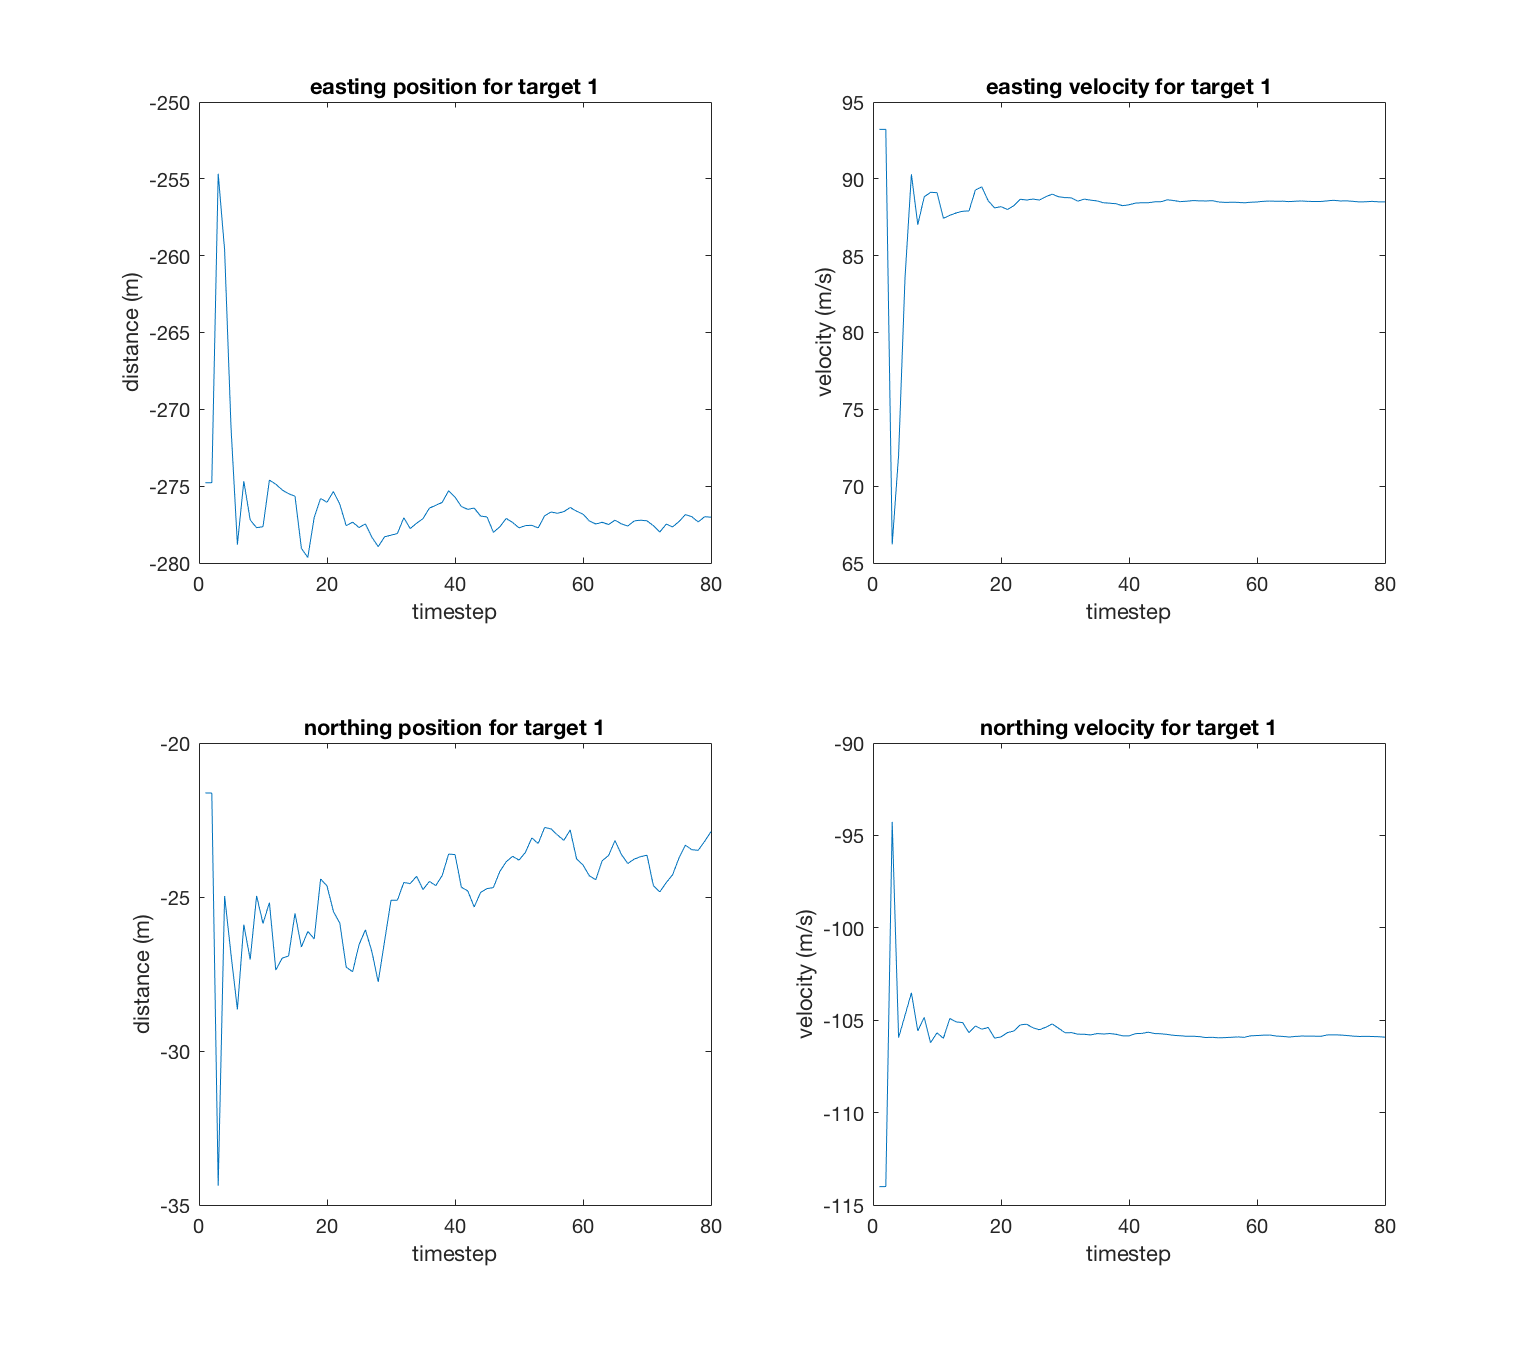
\includegraphics[width=0.8\textwidth]{prob3c_plt1.png}
	\caption{Estimate of initial conditions for aircraft 1}
	\label{xA0}
\end{figure}
\begin{figure}[h]
	\centering
	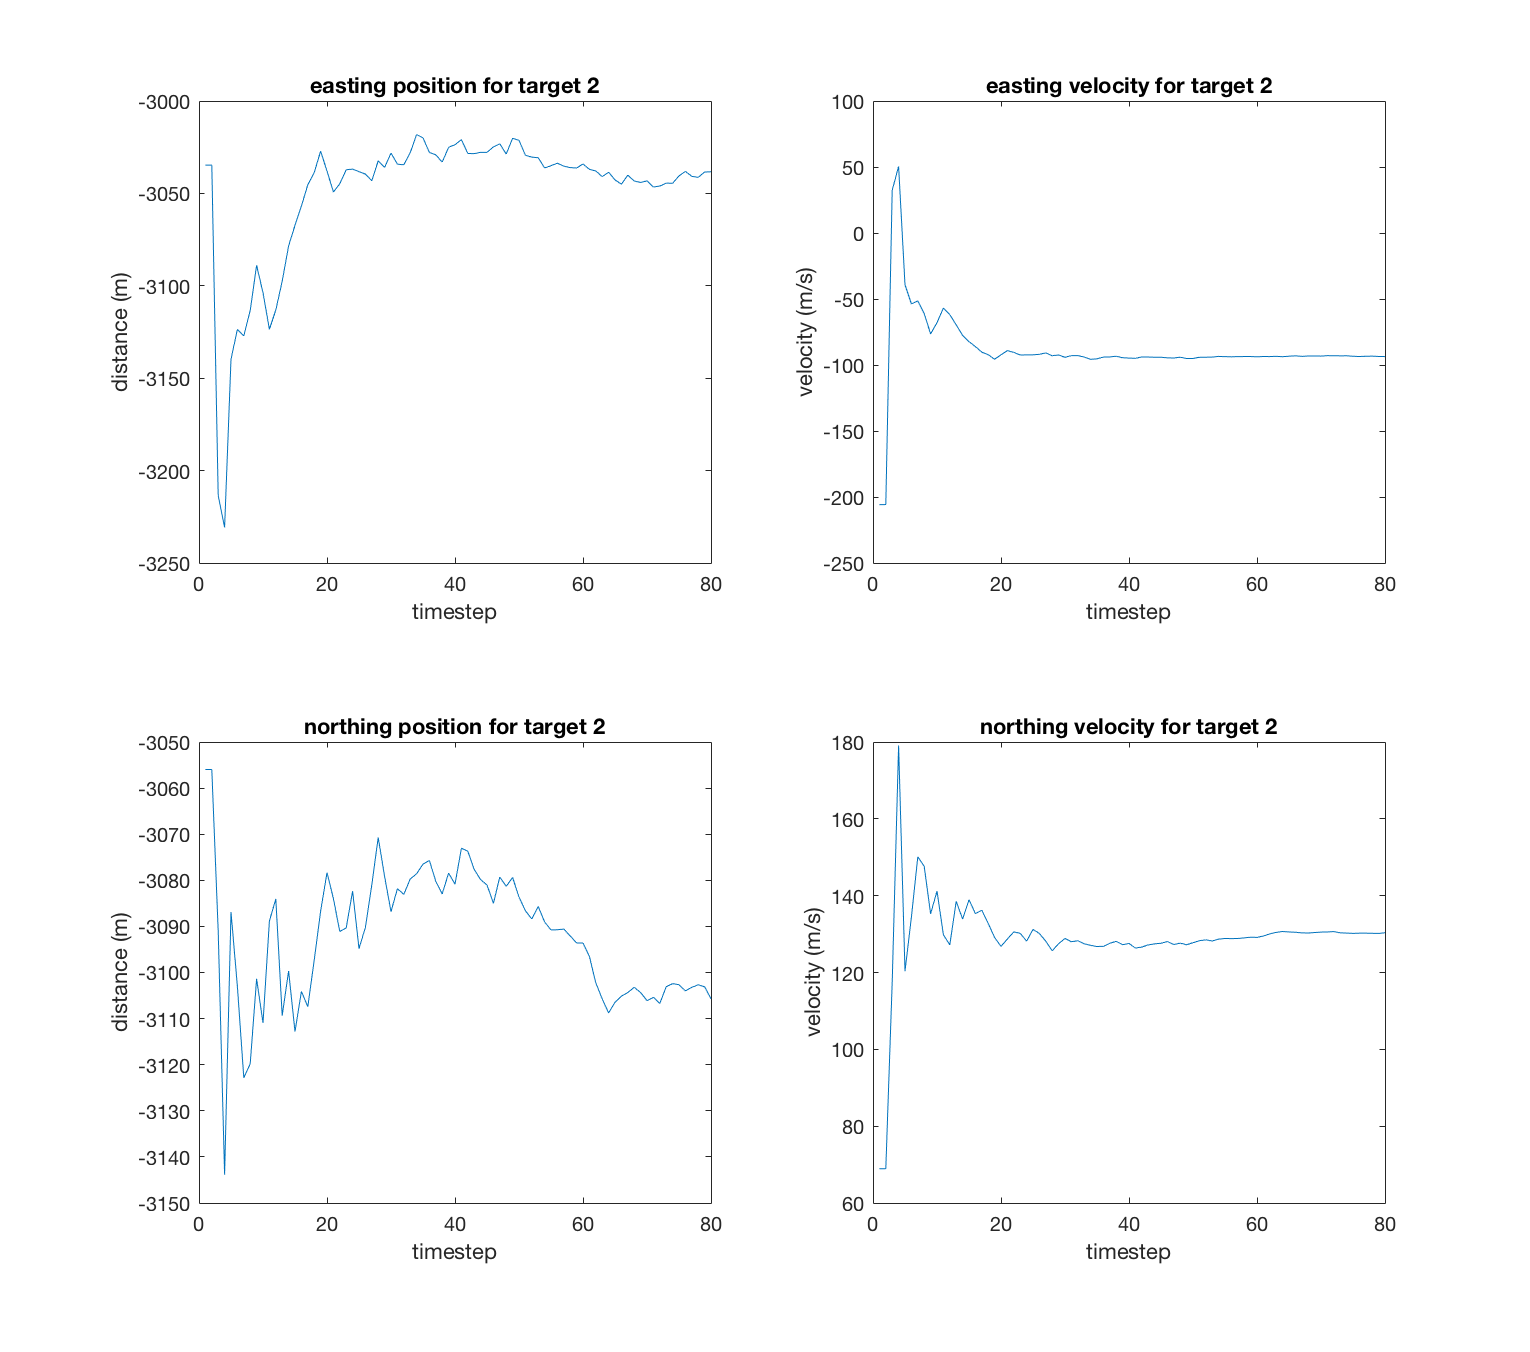
\includegraphics[width=0.8\textwidth]{prob3c_plt2.png}
	\caption{Estimate of initial conditions for aircraft 2}
	\label{xB0}
\end{figure}
\begin{figure}[h]
	\centering
	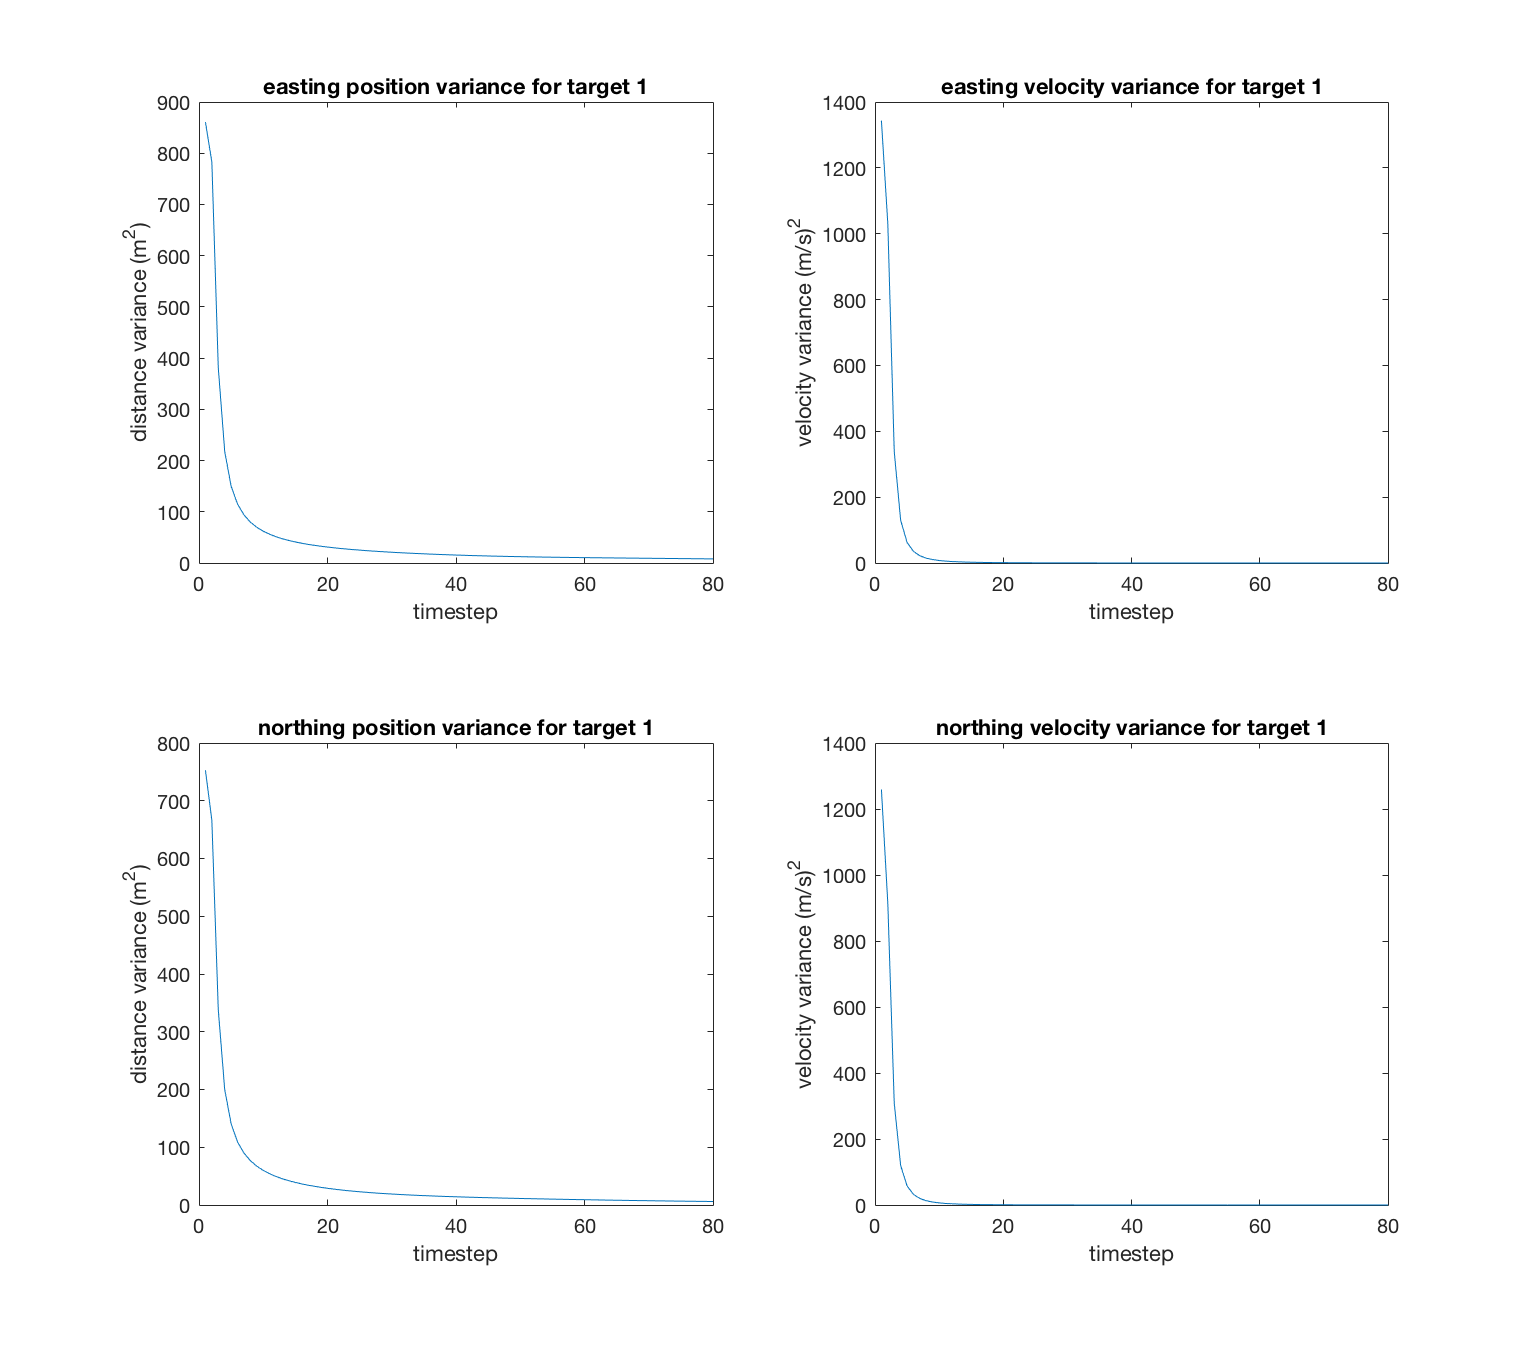
\includegraphics[width=0.8\textwidth]{prob3c_plt3.png}
	\caption{Variance of initial condition estimate for aircraft 1}
	\label{sigmaA}
\end{figure}
\begin{figure}[h]
	\centering
	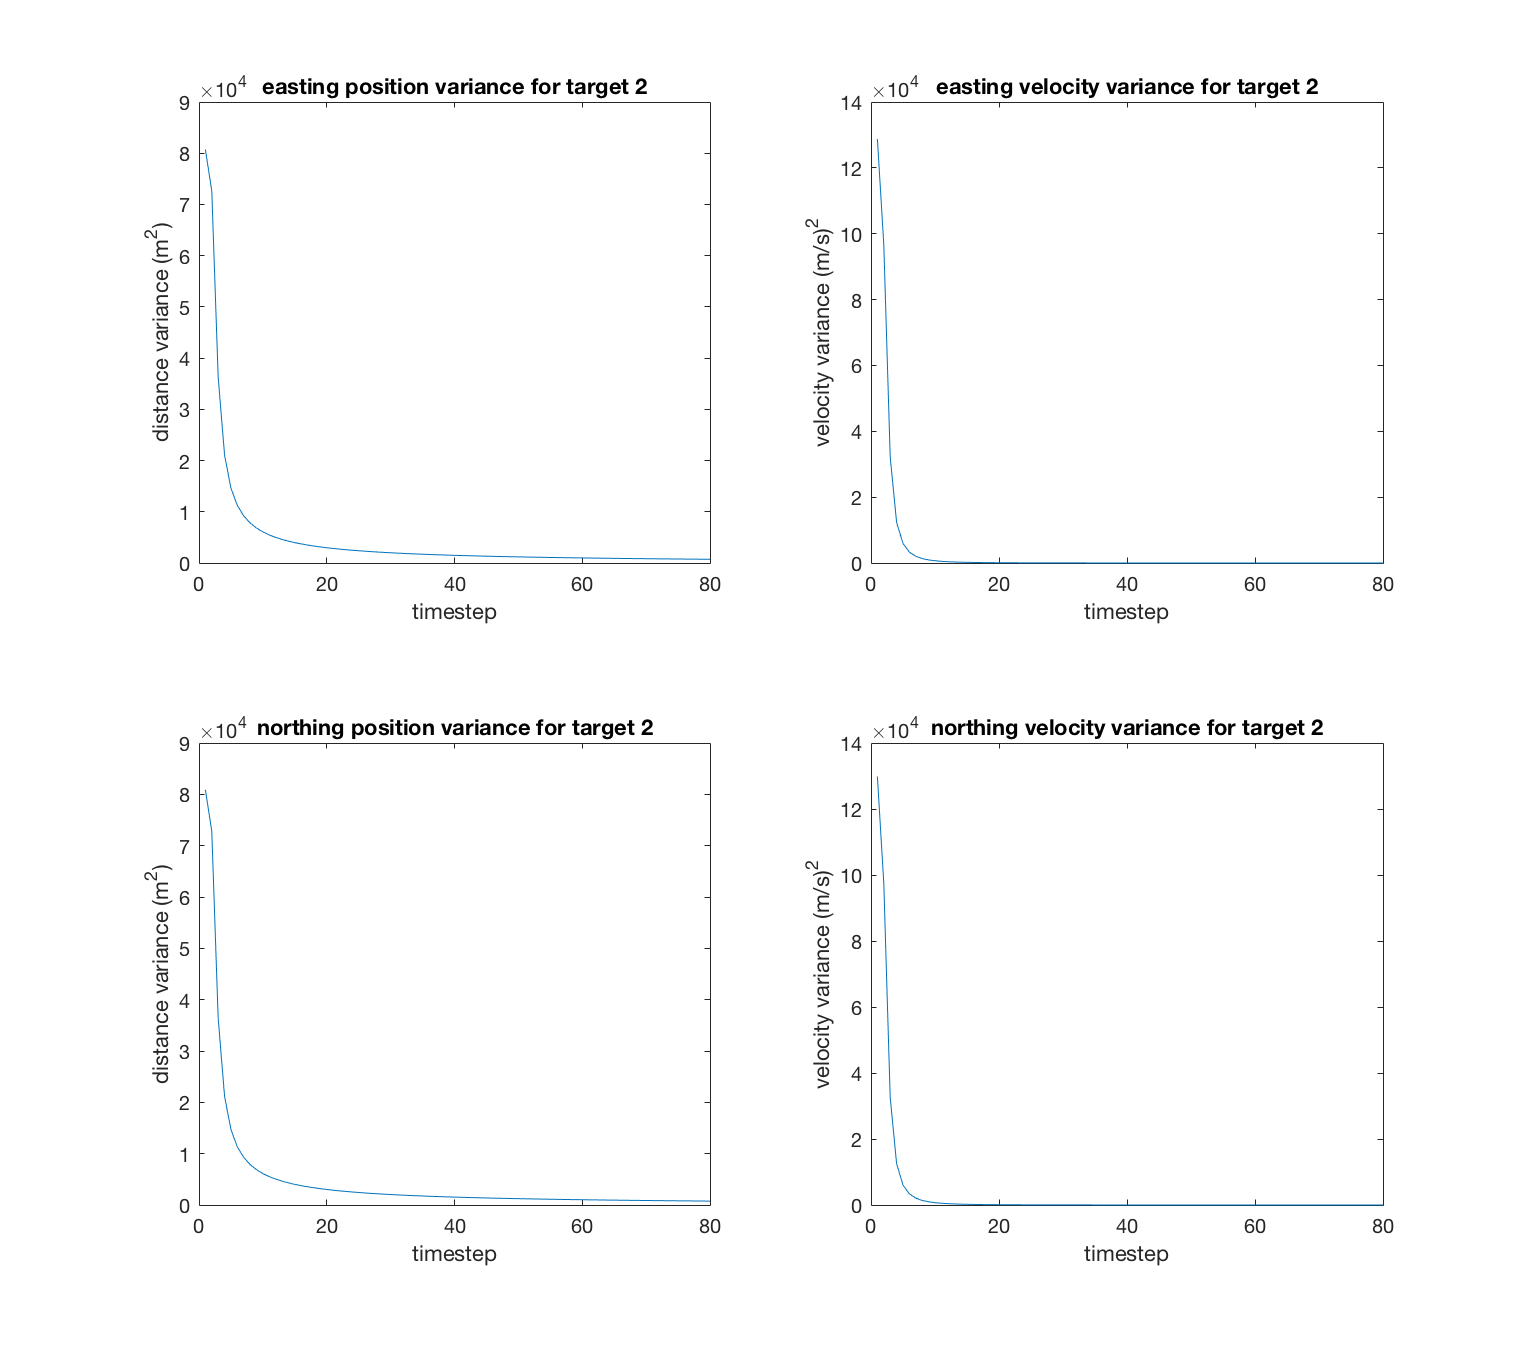
\includegraphics[width=0.8\textwidth]{prob3c_plt4.png}
	\caption{Variance of initial condition estimate for aircraft 2}
	\label{sigmaB}
\end{figure}

\section*{Problem 4}
Consider the pure prediction update for the state covariance of a DT linear Gaussian system with state transition matrix $F$ and process noise covariance matrix $Q$,
\begin{equation*}
	P_{k+1} = FP_kF^T + Q
\end{equation*}
If $F$ is stable, then as $k\rightarrow \infty$, this equation leads to a DT \textit{Lyapunov equation} for the steady-state covariance $P_\infty$,
\begin{equation*}
	P_\infty=FP_\infty F^T + Q
\end{equation*}

\subsection*{part (a)}
Suppose $F=f$ is some scalar constant, where $|f|<1$, and $Q=q$ is an arbitrary process noise variance, with $q>0$. Derive an analytical solution for the scalar steady state covariance $P_\infty=\sigma_\infty^2$.

\subparagraph*{}
\begin{align*}
	\sigma_\infty^2&=\sigma_\infty^2f^2+q \\
	\sigma_\infty^2(1-f^2)&=q \\
	\sigma_\infty^2 &= \frac{q}{1-f^2}
\end{align*}

\subsection*{part (b)}
Run and report (using suitably labeled/scaled plots) a simple simulation of the covariance prediction update for 50 time steps at values of $f=0.8$, $q=10$, and $\sigma_0^2=50$, and compare this to the analytical result from part (a). Repeat and report the comparison for $\sigma_0^2=10$. What do these sets of results tell you about the sensitivity of the steady state variance on the initial variance ot time 0?

\subparagraph*{}
With $\sigma_0^2=50$, $\sigma_{50}^2=27.7777777823$, while $\sigma_\infty^2=27.7777777777$. When $\sigma_0^2=10$, $\sigma_{50}^2=27.7777777774$. This shows the steady state variance is not dependent on the initial variance value.

\subsection*{part (c)}
Now suppose $F$ is an arbitrary non-diagonal but stable $2\times2$ state transition matrix and $Q$ is an arbitrary non-diagonal $2\times2$ covariance matrix. Manually derive an analytical expression for a system of linear equations that provides the solution for the elements of $P_\infty$ in terms of the elements of $F$ and $Q$. You do not need to explicitly solve for each unknown $P_\infty$ element, but you must specify all coefficients for each equation corresponding to the unknown $P_\infty$ elements, and express these together in an appropriate matrix-vector form (don't use a symbolic solver). \textbf{Hint:} the fact that $P_\infty$ and $Q$ are both covariance matrices makes it easy to describe their elements.

\subparagraph*{}
The lyapunov equation for $2\times2$ $F$, $Q$, and $P_\infty$ matrices can be expanded as follows, taking advantage of the fact that $\sigma_{1,2}^2=\sigma_{2,1}^2$ and $q_{1,2}=q_{2,1}$ because $Q$ and $P_\infty$ are covariance matrices and are therefore symmetric.
\begin{align*}
	P_\infty &= FP_\infty F^T + Q \\
	&= \begin{bmatrix} f_{1,1}&f_{1,2}\\f_{2,1}&f_{2,2} \end{bmatrix} \begin{bmatrix} \sigma_{1,1}^2 & \sigma_{1,2}^2 \\ \sigma_{1,2}^2 & \sigma_{2,2}^2 \end{bmatrix} \begin{bmatrix} f_{1,2}&f_{2,1}\\f_{1,2}&f_{2,2} \end{bmatrix} + \begin{bmatrix} q_{1,1} & q_{1,2} \\ q_{1,2} & q_{2,2} \end{bmatrix} \\
	\sigma_{1,1}^2 &= f_{1,1}^2\sigma_{1,1}^2+2f_{1,1}f_{1,2}\sigma_{1,2}^2 + f_{1,2}^2\sigma_{2,2}^2 + q_{1,1} \\
	\sigma_{1,2}^2 &= f_{2,1}f_{1,1}\sigma_{1,1}^2+f_{2,1}f_{1,2}\sigma_{1,2}^2+f_{2,2}f_{1,1}\sigma_{1,2}^2+f_{2,2}f_{1,2}\sigma_{2,2}^2 + q_{1,2} \\
	\sigma_{2,2}^2 &= f_{2,1}^2\sigma_{1,1}^2+2f_{2,1}f_{2,2}\sigma_{1,2}^2+f_{2,2}^2\sigma_{2,2}^2 + q_{2,2}
\end{align*}
The above equations can be solved for the sigmas as follows:
\begin{align*}
	\sigma_{1,1}^2 &= -f_{2,2}(2f_{1,2}q_{1,2}(f_{1,1}f_{2,2} - f_{1,2}f_{2,1}) + f_{2,2}q_{1,1}(-f_{1,1}f_{2,2} + f_{1,2}f_{2,1} + 1)) \\
	&\qquad /(2f_{1,1}^2f_{1,2}f_{2,1}f_{2,2}^2 - 4f_{1,1}f_{1,2}^2f_{2,1}^2f_{2,2} + f_{1,2}^2f_{2,1}^2(f_{1,1}f_{2,2} + f_{1,2}f_{2,1} - 1) \\
	&\qquad + 2f_{1,2}f_{2,1}f_{2,2}^2(f_{1,1}^2 - 1) - f_{2,2}^2(f_{1,1}^2 - 1)(f_{1,1}f_{2,2} + f_{1,2}f_{2,1} - 1)) \\
	\sigma_{1,2}^2 &= -(f_{2,1}f_{2,2}q_{1,1}(f_{1,1}f_{2,2} - f_{1,2}f_{2,1}) + q_{1,2}(f_{1,2}^2f_{2,1}^2 - f_{2,2}^2(f_{1,1}^2 - 1))) \\
	&\qquad /(2f_{1,1}^2f_{1,2}f_{2,1}f_{2,2}^2 - 4f_{1,1}f_{1,2}^2f_{2,1}^2f_{2,2} + f_{1,2}^2f_{2,1}^2(f_{1,1}f_{2,2} + f_{1,2}f_{2,1} - 1) \\
	&\qquad+ 2f_{1,2}f_{2,1}f_{2,2}^2(f_{1,1}^2 - 1) - f_{2,2}^2(f_{1,1}^2 - 1)(f_{1,1}f_{2,2} + f_{1,2}f_{2,1} - 1)) \\
	\sigma_{2,2}^2 &= f_{2,1}(f_{2,1}q_{1,1}(f_{1,1}f_{2,2} - f_{1,2}f_{2,1} + 1) + 2q_{1,2}(f_{1,1}f_{1,2}f_{2,1} - f_{2,2}(f_{1,1}^2 - 1))) \\
	&\qquad /(2f_{1,1}^2f_{1,2}f_{2,1}f_{2,2}^2 - 4f_{1,1}f_{1,2}^2f_{2,1}^2f_{2,2} + f_{1,2}^2f_{2,1}^2(f_{1,1}f_{2,2} + f_{1,2}f_{2,1} - 1) \\
	&\qquad+ 2f_{1,2}f_{2,1}f_{2,2}^2(f_{1,1}^2 - 1) - f_{2,2}^2(f_{1,1}^2 - 1)(f_{1,1}f_{2,2} + f_{1,2}f_{2,1} - 1))
\end{align*}
These equations can be rewritten in linear algebra terms as
\begin{equation*}
	P_\infty = \sum_{i=0}^\infty F^iQ(F^T)^i
\end{equation*}

\subsection*{part (d)}
Use the result from part (c) to solve for the elements of $P_\infty$ for the following $F$ and $Q$ values:
\begin{equation*}
	F=\begin{bmatrix} 0.99&0.2\\0&-0.76 \end{bmatrix}\quad Q=\begin{bmatrix} 1&0.37\\0.37&2.5 \end{bmatrix}
\end{equation*}

\subparagraph*{}
Using the summation from part (c) we find 
\begin{equation*}
	P_\infty = \begin{bmatrix} 56.13 & -0.3022 \\ -0.3022 & 5.919 \end{bmatrix}
\end{equation*}

\subsection*{part (e)}
Use suitably labeled/scaled plots to validate your results from part (d) by comparing to both (a) a sufficiently long predicted covariance simulation for $P_0=10\cdot I_{2\times 2}$, and (b) the output of the \texttt{dlyap.m} command in Matlab.

\subparagraph*{}
The evolution of $\sigma_{1,1}^2$ over the simulation or summation iteration is shown below in figure \ref{sig11}. Similarly, figures \ref{sig12} and \ref{sig22} show the same information for $\sigma_{1,2}^2$ and $\sigma_{2,2}^2$ respectively. It is interesting to note the analytical and simulated methods converge at roughly the same rate and both converge to the value given by \texttt{dlyap.m}.
\begin{figure}[h]
	\centering
	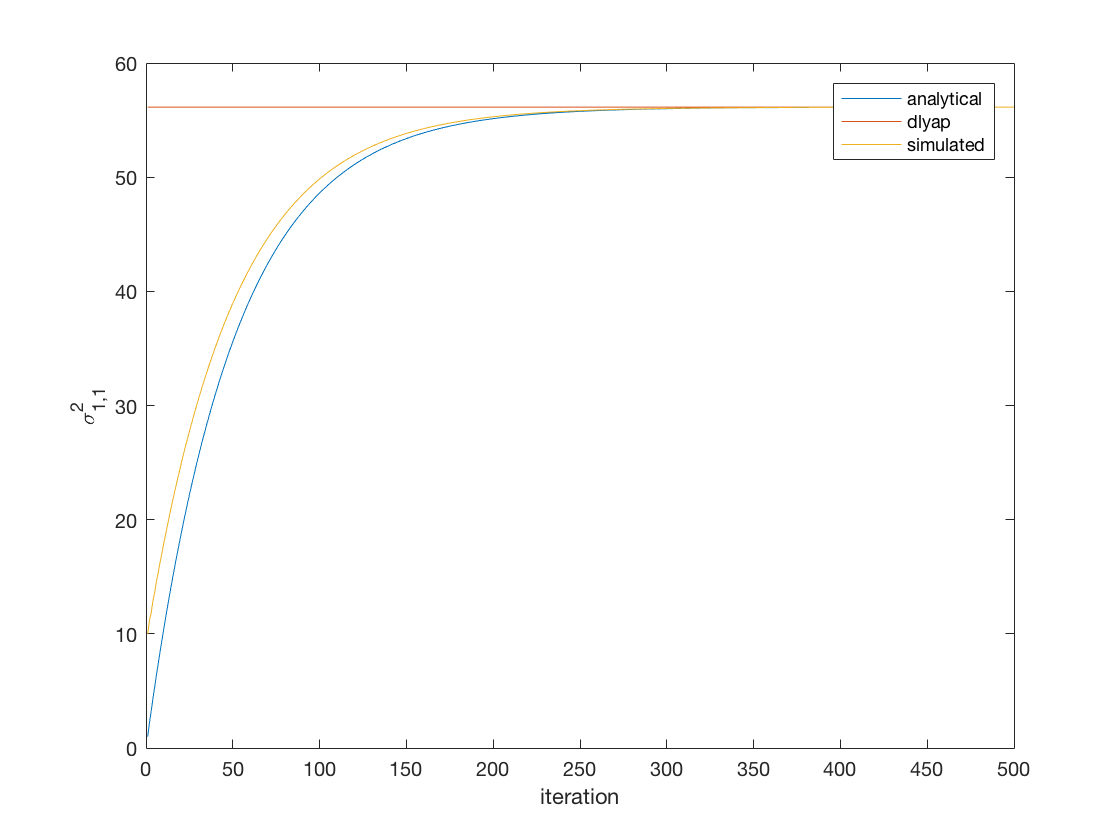
\includegraphics[width=0.8\textwidth]{prob4e_plt1.png}
	\caption{Evolution of $\sigma_{1,1}^2$ for analytical and simulated solutions}
	\label{sig11}
\end{figure}

\begin{figure}[h]
	\centering
	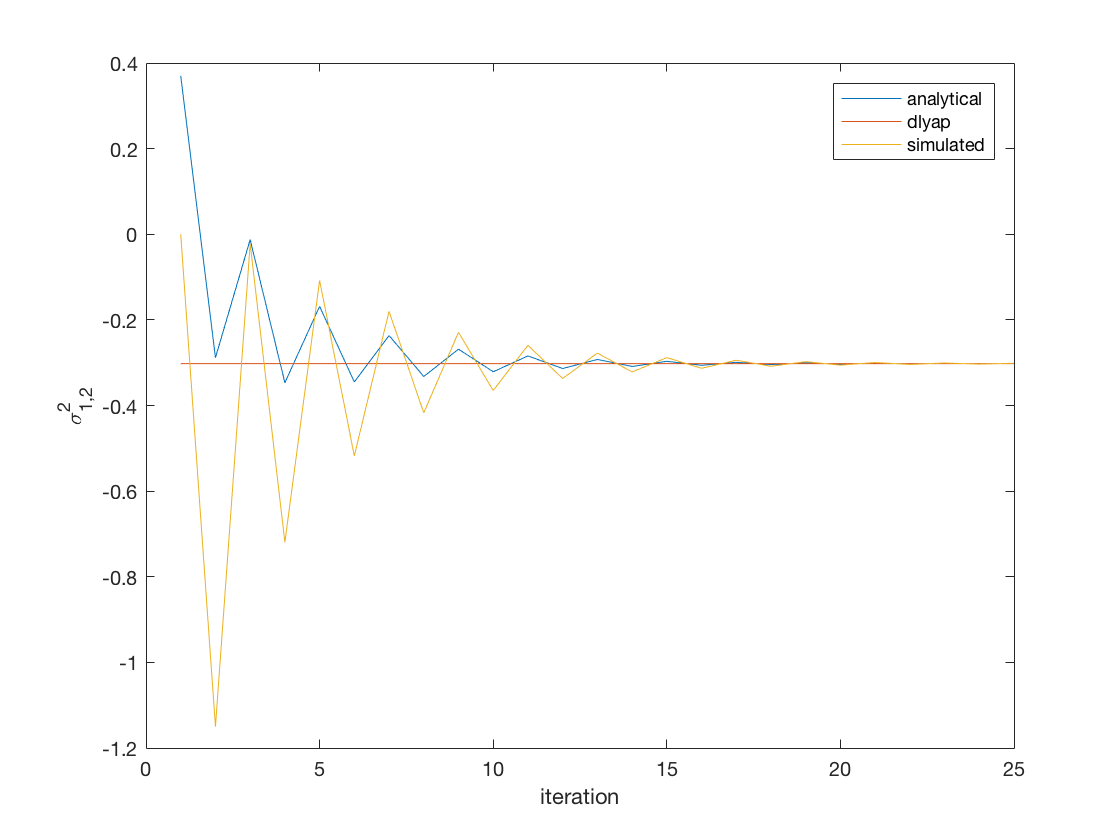
\includegraphics[width=0.8\textwidth]{prob4e_plt2.png}
	\caption{Evolution of $\sigma_{1,2}^2$ for analytical and simulated solutions}
	\label{sig12}
\end{figure}

\begin{figure}[h]
	\centering
	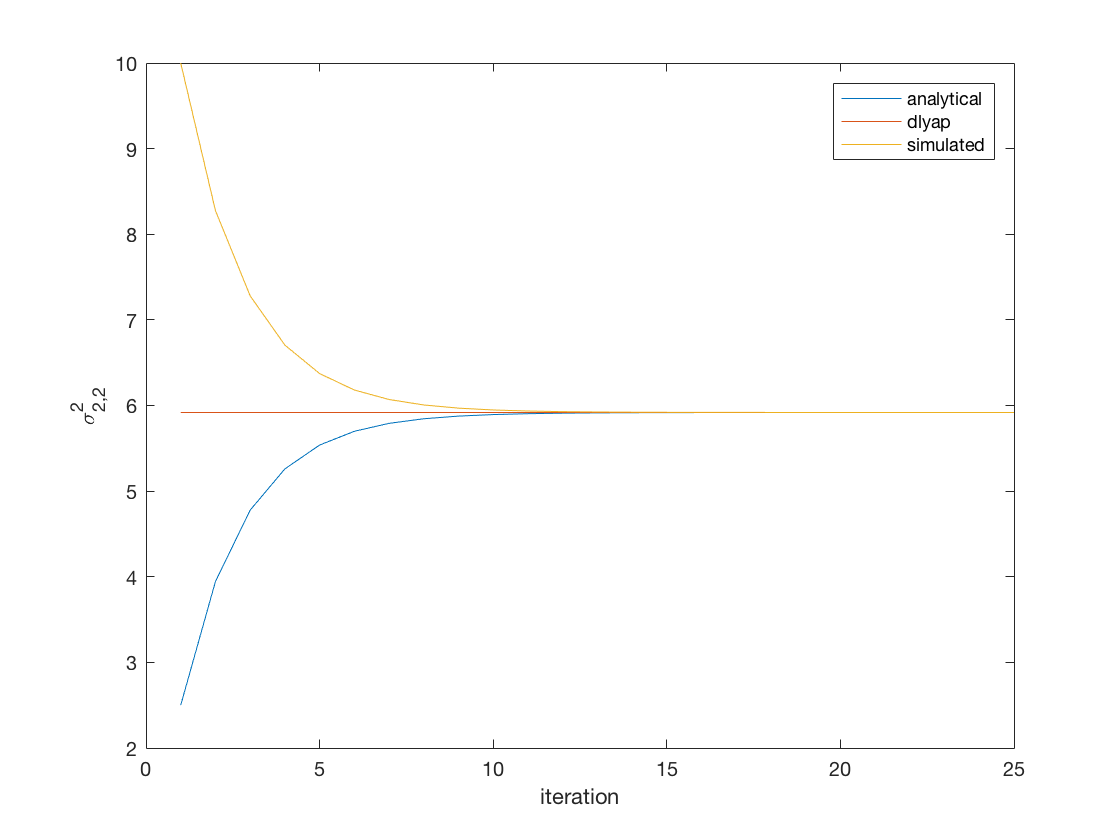
\includegraphics[width=0.8\textwidth]{prob4e_plt3.png}
	\caption{Evolution of $\sigma_{2,2}^2$ for analytical and simulated solutions}
	\label{sig22}
\end{figure}

\end{document}

